\section{Time complexity of operations}
\label{sec:time_complexity_of_operations}

\begin{frame}
	\frametitle{Did we improve?}
	\framesubtitle{\url{http://tmbw.net/wiki/File:Speed_And_Velocity.png}}
	\begin{center}
		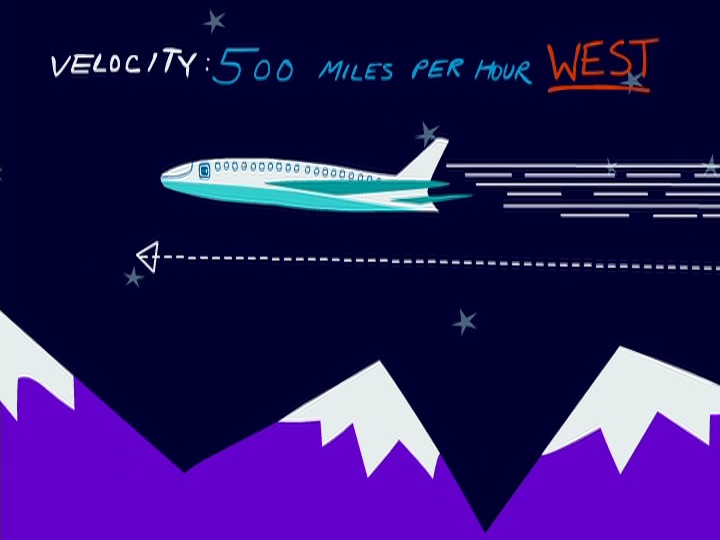
\includegraphics[width=0.6\textwidth]{figures/speed.png}\\
		\hspace*{15pt}\hbox{\scriptsize Image By:\thinspace{\itshape They Might be Giants}}
	\end{center}
\end{frame}

\begin{frame}
	\frametitle{An observation of heaps}
	
	\begin{questionblock}{Height of a heap}
		Remember that for a tree, we had worst-case $h = n$. But what about a heap?
		\begin{itemize}
			\item $h$ is $\Theta(\log \log n)$
			\item $h$ is $\Theta(\log n)$
			\item $h$ is $\Theta(n)$
			\item $h$ is $\Theta(n^2)$
		\end{itemize}
	\end{questionblock}
	\pause
	\begin{answerblock}{Balanced trees}
		Remember that it is balanced and complete, meaning the height is $\Theta(\log n)$!
	\end{answerblock}
\end{frame}

\begin{frame}
	\frametitle{So how does our heap-based PQ do?}

		\begin{exampleblock}{Single path}
			Both operations bubble up or down one path, so both are $\Theta(\log n)$.\\
			A good improvement over the $\Theta(n)$ array-based implementations.
		\end{exampleblock}	
		\pause
		\begin{questionblock}{Decreasing keys}
			We can also decrease the value of an item in $\Theta(\log n)$ time (how?), but we cannot increase the value of an
			item in $\Theta(\log n)$ time. Why not?
		\end{questionblock}
		\pause
		\begin{answerblock}{Going up, going down}
			Going up the heap is easy, so smaller keys can be moved up.\\
			But going down the heap is way harder, because we need to end up on the bottom right of the heap. Repeatedly
			switching with the smaller of the two below us, could lead to issues. (example on smartboard)
		\end{answerblock}
		\pnote{8 - (12,24) - ((13,14),(22,25)), update 8 to 12}
	
\end{frame}

\begin{frame}
	\frametitle{So the PQ}
	
	\begin{center}
		\begin{tabular}{r | c  c c}
			PriorityQueue & Array-based & Sorted Array & Heap-based \\
			\midrule
			\texttt{size()} & $O(1)$ & $O(1)$ & $O(1)$ \\
			\texttt{add(item)}& $O(1)\footnote{amortised}$ &$O(n)$ & $O(\log n)$ \\
			\texttt{remove\_min()}& $O(n)$ &$O(n)$ & $O(\log n)$ \\
			\texttt{min()}& $O(n)$ &$O(1)$ & $O(1)$ \\
		\end{tabular}
	\end{center}
	\begin{itemize}
		\item Heap-based PQ's are clearly the best!
		\item There are no downsides?
			\pause
		\item Except for a little more space due to the heap structure, over just an array.
			\pause
		\item We can do even better with Fibonacci-heaps (not this course).
	\end{itemize}
\end{frame}
